
\documentclass[10pt, letterpaper]{article}

% package used to set margins, adjust parameters with caution
\usepackage[left = 0.70in, right = 0.70in, top = 1.0in, bottom = 1.5in]{geometry}

%%%%%%%%%%%%%%%%%%%%%%%%%%%%%%%%%%%%%%%%%%%%%%
%%%%%%%%%%%%%%%%%%%%%%%%%%%%%%%%%%%%%%%%%%%%%%

% package used to include special header and footer formatting
\usepackage{fancyhdr}

% package used to include special formatting for image and table captions
\usepackage[small,bf,justification=raggedright,format=hang]{caption}

\usepackage{amscd}
\usepackage{amsfonts}
\usepackage{amsmath}
\usepackage{amssymb}

\usepackage{color}
\usepackage[usenames,dvipsnames]{xcolor}
\usepackage{epsfig}
\usepackage{graphicx}
\usepackage{multicol}
\usepackage{verbatim}
\usepackage{relsize}
\usepackage{tikz}
\usetikzlibrary{arrows,decorations.markings}
%\usepackage{doublespace}

%%%%%%%%%%%%%%%%%%%%%%%%%%%%%%%%%%%%%%%%%%%%%%
%%%%%%%%%%%%%%%%%%%%%%%%%%%%%%%%%%%%%%%%%%%%%%
\renewcommand{\theenumi}{\arabic{enumi}}
\renewcommand{\labelenumi}{\mbox{}\;\theenumi.$\;$}

\renewcommand{\theenumii}{\alph{enumii}}
\renewcommand{\labelenumii}{\mbox{}\;\;\,\theenumii)$\quad$}

\renewcommand{\theenumiii}{\roman{enumiii}}
\renewcommand{\labelenumiii}{\mbox{}\;\;\,\theenumiii)$\quad$}

\renewcommand{\theequation}{\thesection .\arabic{equation}}

\newcounter{theorem}

\newtheorem{example}[theorem]{Example}
\renewcommand{\theexample}{ \thesection .\arabic{example}}

\newtheorem{definition}[theorem]{Definition}
\renewcommand{\thedefinition}{\thesection .\arabic{definition}}

\newtheorem{theorem}[theorem]{Theorem}
\renewcommand{\thetheorem}{\thesection .\arabic{theorem}}

\newtheorem{proposition}[theorem]{Proposition}
\renewcommand{\theproposition}{\thesection .\arabic{proposition}}

\newtheorem{conjecture}[theorem]{Conjecture}
\renewcommand{\theconjecture}{\thesection .\arabic{conjecture}}

\newtheorem{lemma}[theorem]{Lemma}
\renewcommand{\thelemma}{\thesection .\arabic{lemma}}

\newtheorem{corollary}[theorem]{Corollary}
\renewcommand{\thecorollary}{\thesection .\arabic{corollary}}

\newtheorem{remark}[theorem]{Remark}
\renewcommand{\theremark}{\thesection .\arabic{remark}}

\newtheorem{notation}[theorem]{Notation}
\renewcommand{\thenotation}{\thesection .\arabic{notation}}

\renewcommand{\thetable} {\thesection .\arabic{table}}

\renewcommand{\thefigure}{\thesection .\arabic{figure}}

%%%%%%%%%%%%%%%%%%%%%%%%%%%%%%%%%%%%%%%%%%%%%%
%%%%%%%%%%%%%%%%%%%%%%%%%%%%%%%%%%%%%%%%%%%%%%
\newcommand*{\proof}{\noindent {\small P{\scriptsize ROOF}} \quad}
\newcommand*{\proofof}{\noindent {\small P{\scriptsize ROOF OF }}}
\newcommand*{\proofoutline}{\noindent {\small O{\scriptsize UTLINE OF PROOF}} \quad}
\newcommand*{\proofoutlineof}{\noindent {\small O{\scriptsize UTLINE OF PROOF OF }}}
\newcommand*{\qed}{\hfill $\Box$}
\newcommand*{\hdiamond}{\hfill $\Diamond$}

\newcommand{\wconverge}{\rightsquigarrow}

\newcommand*{\D}{\mathbb{D}}
\renewcommand*{\Re}{\mathbb{R}}
\renewcommand*{\d}{\textnormal{d}}
\newcommand{\G}{\mathbb{G}}
\newcommand{\E}{\mathbb{E}}
\newcommand{\C}{\mathbb{C}}
\newcommand{\Q}{\mathbb{Q}}
\newcommand{\N}{\mathbb{N}}
\newcommand{\Z}{\mathbb{Z}}
\newcommand{\F}{\mathbb{F}}
\newcommand{\varemptyset}{\varnothing}
\renewcommand{\i}{\textnormal{\bf i}}

\newcommand{\diag}{\textnormal{diag}}
\newcommand{\proj}{\textnormal{proj}}
\newcommand{\rot}{\textnormal{rot}}

\newcommand{\ev}{\textnormal{ev}}
\newcommand{\rank}{\textnormal{rank}}
\renewcommand*{\span}{\textnormal{span}}
\newcommand*{\domain}{\textnormal{domain}}
\newcommand*{\codomain}{\textnormal{codomain}}
\newcommand{\Col}{\textnormal{Col}}
\newcommand{\image}{\textnormal{image}}
\newcommand{\Var}{\textnormal{Var}}
%\newcommand{\Hess}{\textnormal{Hess}}
\newcommand{\Hess}{\nabla^{2}}
\newcommand{\Cov}{\textnormal{Cov}}
\newcommand{\MSE}{\textnormal{MSE}}
\newcommand{\SVar}{\textnormal{SVar}}
\newcommand{\argmax}{\textnormal{argmax}}
\newcommand{\zeros}{\textnormal{zeros}}

\newcommand*{\longhookrightarrow}{\ensuremath{\lhook\joinrel\relbar\joinrel\rightarrow}}

%\newcommand{\Czo}{C([0,1],\Re)}
\newcommand{\Czo}{C[0,1]}

\newcommand{\logisticBetaX}{
	\dfrac{\exp\!\left(\,\beta^{T} \cdot x \,\right)}{1 \,+\, \exp\!\left(\,\beta^{T} \cdot x \,\right)}
}

\newcommand{\oneMinusLogisticBetaX}{
	\dfrac{1}{1 \,+\, \exp\!\left(\,\beta^{T} \cdot x \,\right)}
}

%%%%%%%%%%%%%%%%%%%%%%%%%%%%%%%%%%%%%%%%%%%%%%
%%%%%%%%%%%%%%%%%%%%%%%%%%%%%%%%%%%%%%%%%%%%%%

\begin{document}

%%%%%%%%%%%%%%%%%%%%%%%%%%%%%%%%%%%%%%%%%%%%%%

%\setcounter{page}{1}

\pagestyle{fancy}

\rhead[Study Notes]{Kenneth Chu}
\lhead[Kenneth Chu]{Study Notes}
\chead[]{{\Large\bf PCA Stability Assessment via the bootstrap and Grassmannians} \\
\vskip 0.1cm \normalsize \today}
\lfoot[]{}
\cfoot[]{}
\rfoot[]{\thepage}

%%%%%%%%%%%%%%%%%%%%%%%%%%%%%%%%%%%%%%%%%%%%%%

          %%%%% ~~~~~~~~~~~~~~~~~~~~ %%%%%

{\color{white}.}
\vskip -0.95cm
{\color{white}.}

          %%%%% ~~~~~~~~~~~~~~~~~~~~ %%%%%

\section{The operator norm of the difference of two Euclidean orthogonal projection operators is 1}
\setcounter{theorem}{0}
\setcounter{equation}{0}

%\cite{vanDerVaart1996}
%\cite{Kosorok2008}

%\renewcommand{\theenumi}{\alph{enumi}}
%\renewcommand{\labelenumi}{\textnormal{(\theenumi)}$\;\;$}
\renewcommand{\theenumi}{\roman{enumi}}
\renewcommand{\labelenumi}{\textnormal{(\theenumi)}$\;\;$}

          %%%%% ~~~~~~~~~~~~~~~~~~~~ %%%%%

\begin{proposition}
\mbox{}\vskip 0.1cm
\noindent
Suppose:
\begin{itemize}
\item
	$n \in \N$\, is a positive integer.
\item
	$\Re^{n}$\, is the $n$-dimensional inner product space over $\Re$ equipped with the standard Euclidean inner product.
\item
	$P_{1}, \, P_{2} \, : \, \Re^{n} \, \longrightarrow \, \Re^{n}$\,
	are nonzero orthogonal projection operators on $\Re^{n}$.
\item
	$\left\Vert\; P_{1} \overset{{\color{white}.}}{-} P_{2} \;\right\Vert$\,
	is the operator norm (induced by the Euclidean norm on $\Re^{n}$)
	of the difference operator \,$P_{1} - P_{2}$, i.e.
	\begin{equation*}
	\left\Vert\; P_{1} \overset{{\color{white}.}}{-} P_{2} \;\right\Vert
	\;\; := \;\;
		\sup\,\left\{\;\;
			\left\Vert\;(\,P_{1} \overset{{\color{white}.}}{-} P_{2}\,) \cdot v \;\right\Vert \,\geq\, 0
			\;\;\left\vert\;
			\begin{array}{c}
				{\color{white}..}v \in \Re^{n} \\ \Vert\,v\,\Vert = 1
				\end{array}
			\right.\right\}
	\end{equation*}
\end{itemize}
Then,
\begin{equation*}
\left\Vert\; P_{1} \overset{{\color{white}.}}{-} P_{2} \;\right\Vert
\;\; \leq \;\;
	1
\end{equation*}
\end{proposition}
\proof
We need to establish that
\begin{equation}\label{wantToProve}
\left\Vert\;\, (\,P_{1} \,\overset{{\color{white}.}}{-}\, P_{2}\,)\cdot v \,\;\right\Vert
\;\; \leq \;\;
	1\,,
\quad
\textnormal{for each unit vector \,$v \in \Re^{n}$}\,.
\end{equation}
First, note that, for an arbitrary unit vector \,$v \in \Re^{n}$,\,
if \,$P_{1} \cdot v = 0$\,,\, then
\begin{equation*}
\left\Vert\;\, (\,P_{1} \,\overset{{\color{white}.}}{-}\, P_{2}\,)\cdot v \,\;\right\Vert
\;\; = \;\;
	\left\Vert\;\, P_{2} \overset{{\color{white}.}}{\cdot} v \,\;\right\Vert
\;\; \leq \;\;
	\left\Vert\;\, P_{2} \,\;\right\Vert
	\cdot
	\left\Vert\, v \,\;\right\Vert
\;\; = \;\;
	1 \cdot 1
\;\; = \;\;
	1
\end{equation*}
Simillarly,
\begin{equation*}
P_{2} \cdot v = 0
\quad\Longrightarrow\quad
\left\Vert\;\, (\,P_{1} \,\overset{{\color{white}.}}{-}\, P_{2}\,)\cdot v \,\;\right\Vert
\;\; = \;\;
	\left\Vert\;\, P_{1} \overset{{\color{white}.}}{\cdot} v \,\;\right\Vert
\;\; \leq \;\;
	\left\Vert\;\, P_{1} \,\;\right\Vert
	\cdot
	\left\Vert\, v \,\;\right\Vert
\;\; = \;\;
	1 \cdot 1
\;\; = \;\;
	1
\end{equation*}
In other words, \eqref{wantToProve} holds whenever
\,$P_{1}\cdot v = 0$\, or \,$P_{2}\cdot v = 0$.\,
Thus, it remains only to establish \eqref{wantToProve}
for an arbitrary unit vector \,$v \in \Re^{n}$\, satisfying:
\begin{equation}\label{caseAssumption}
P_{1} \cdot v \neq 0
\quad\textnormal{and}\quad
P_{2} \cdot v \neq 0\,.
\end{equation}
Hence, let \,$v \in \Re^{n}$\, be an arbitrary such unit vector.
Observe that:
\begin{equation*}
\dim\left(\,\span\left\{\,\overset{{\color{white}-}}{v} \,,\, P_{1}\cdot v \,,\, P_{2}\cdot v\,\right\}\,\right)
\;\; \leq \;\;
	3\,.
\end{equation*}
Hence, we may fix a $3$-dimensional vector subspace \,$V \subset \Re^{n}$\, such that
\begin{equation*}
\span\left\{\,\overset{{\color{white}-}}{v} \,,\, P_{1}\cdot v \,,\, P_{2}\cdot v\,\right\}
\;\; \subset \;\;
	V.
\end{equation*}
Note that \,$V$\, is isomorphic to \,$\Re^{3}$\, as an inner product space,
and by applying a suitable isometry on \,$\Re^{3}$\, if necessary,
we may furthermore fix an inner product isomorphism \,$\Phi : V \longrightarrow \Re^{3}$\,
such that
\begin{equation*}
\Phi(v) = (\,0,0,1) \,\in\, \Re^{3}\,,
\quad\textnormal{and}\quad
\Phi(\,P_{1}\cdot v\,) \in \span\left\{\;(\,\overset{{\color{white}.}}{1},0,0) \,,\, (\,0,0,1)\;\right\}.
\end{equation*}
For such a \,$\Phi$\,, we therefore have:
\begin{eqnarray*}
\Phi(\,P_{1}\cdot v\,)
& = &
	\left(\;
		-\,\cos\theta_{1}\cdot\sin\theta_{1}{\color{white}\cdot\cos\varphi.}
		\; , \;
		0{\color{white}\cos\theta_{1}\cdot\sin\theta_{1}........}
		\; , \;
		\cos\theta_{1}\overset{{\color{white}1}}{\cdot}\cos\theta_{1}
		\;\right)
	\;\;\in\;\; \Re^{3}
\\
\Phi(\,P_{2}\cdot v\,)
& = &
	\left(\;
		{\color{white}-}\,\cos\theta_{2}\cdot\sin\theta_{2}\cdot{\color{red}\cos\varphi}
		\; , \;
		\cos\theta_{2}\cdot\sin\theta_{2}\cdot{\color{red}\sin\varphi}
		\; , \;
		\cos\theta_{2}\overset{{\color{white}1}}{\cdot}\cos\theta_{2}
		\;\right)
	\;\;\in\;\; \Re^{3}
\end{eqnarray*}
for some \,$(\,\theta_{1}, \theta_{2},\varphi\,)$ \,$\in$\,
$\left[\,0\,,\dfrac{\pi}{2}\,\right) \times \left[\,0\,,\dfrac{\pi}{2}\,\right) \times \left[\,0\,,\overset{{\color{white}.}}{2\,\pi}\right)$.
Note in particular that for these admissible values of \,$(\,\theta_{1}, \theta_{2},\varphi\,)$\,, we have:
\begin{equation}\label{sineCosineRestrictions}
0
\;\; \leq \;\;
	\cos\theta_{1} \; , \; \sin\theta_{1} \; , \; \cos\theta_{2} \; , \; \sin\theta_{2}
\;\; \leq \;\;
	1\,,
\quad\quad\textnormal{and}\quad\quad
-1
\;\; \leq \;\;
	\cos\varphi
\;\; \leq \;\;
	1
\end{equation}
\vskip 0.5cm
\noindent
See the following figure for the illustration of the special case where \,$\varphi = 0$ (i.e. $v$, $P_{1}\cdot v$ and $P_{2}\cdot v$ are coplanar):
\begin{center}
\vskip 0.8cm

%%%%%%%%%%

%\begin{figure}[h]

\centering
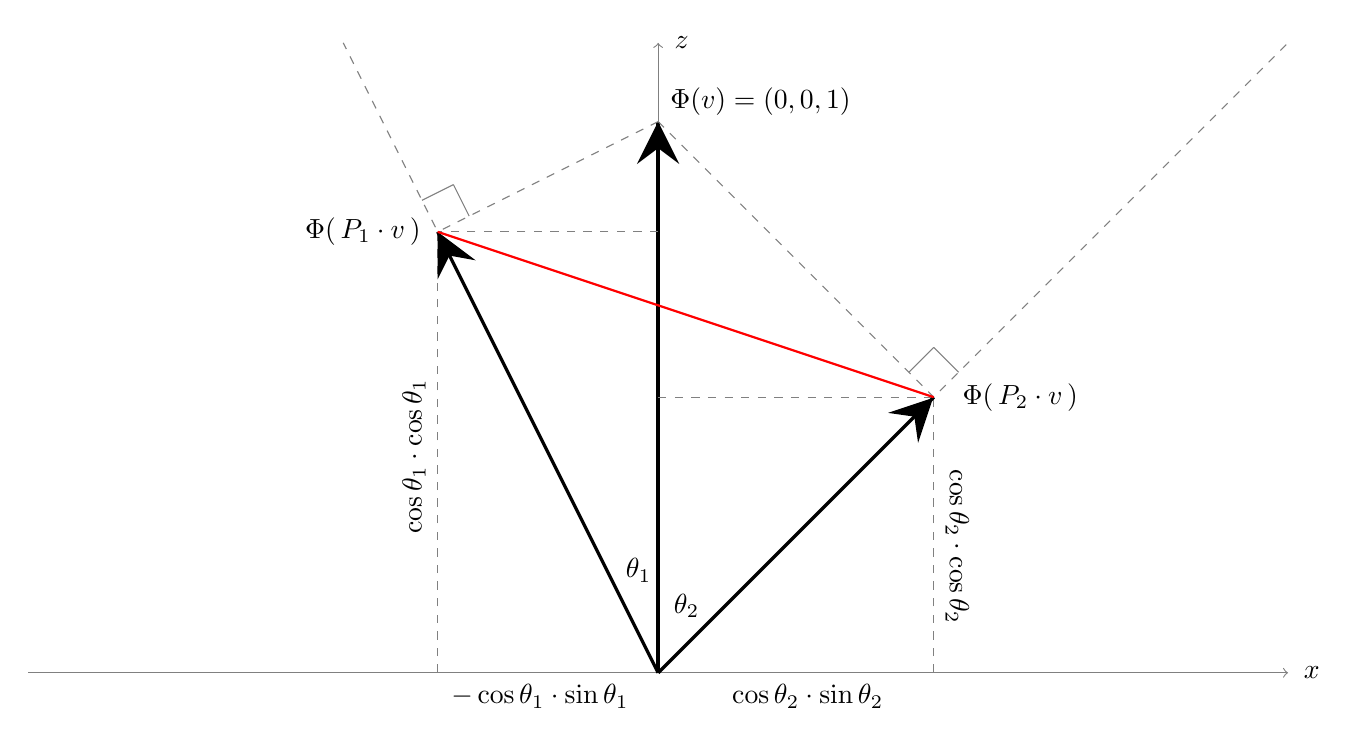
\begin{tikzpicture}

%%%  ~~~~~~~~~~  %%%
% axes
\node at (8.3,0) {$x$};
\node at (0.3,8.0) {$z$};
\draw [->,color=gray] (-8,0) -- (8,0);
\draw [->,color=gray] (0,0) -- (0,8);

%%%  ~~~~~~~~~~  %%%
% (0,0,1)
\node at (1.3,7.25) {$\Phi(v) = (0,0,1)$};
% vector
\draw
	[very thick,decoration={markings,mark=at position 1 with {\arrow[scale=3,>=stealth]{>}}},postaction={decorate}]
	(0,0) -- (0,7);

%%%  ~~~~~~~~~~  %%%
% \Phi( P_{1} cdot v )
\node at (-0.25,1.3) {$\theta_{1}$};
\node at (-3.75,5.6) {$\Phi(\, P_{1} \cdot v \,)$};
\node at (-1.5,-0.3) {$-\cos\theta_{1}\cdot\sin\theta_{1}$};
\node [rotate=90] at (-3.1,2.75) {$\cos\theta_{1}\cdot\cos\theta_{1}$};
\draw [thin,dashed,color=gray] (0,0) -- (-4,8);
\draw [thin,dashed,color=gray] (0,7) -- (-2.8,5.6);
\draw [thin,dashed,color=gray] (-2.8,0) -- (-2.8,5.6);
\draw [thin,dashed,color=gray] (0,5.6) -- (-2.8,5.6);
% right angle symbol
\draw [thin,color=gray] (-3,6) -- (-2.6,6.2);
\draw [thin,color=gray] (-2.4,5.8) -- (-2.6,6.2);
% vector
\draw
	[very thick,decoration={markings,mark=at position 1 with {\arrow[scale=3,>=stealth]{>}}},postaction={decorate}]
	(0,0) -- (-2.8,5.6);

%%%  ~~~~~~~~~~  %%%
% \Phi( P_{2} cdot v )
\node at (0.36,0.85) {$\theta_{2}$};
\node at (4.6,3.5) {$\Phi(\, P_{2} \cdot v \,)$};
\node at (1.9,-0.3) {$\cos\theta_{2}\cdot\sin\theta_{2}$};
\node [rotate=-90] at (3.8,1.6) {$\cos\theta_{2}\cdot\cos\theta_{2}$};
\draw [thin,dashed,color=gray] (0,0) -- (8,8);
\draw [thin,dashed,color=gray] (0,7) -- (3.5,3.5);
\draw [thin,dashed,color=gray] (0,3.5) -- (3.5,3.5);
\draw [thin,dashed,color=gray] (3.5,0) -- (3.5,3.5);
% right angle symbol
\draw [thin,color=gray] (3.184,3.816) -- (3.5,4.132);
\draw [thin,color=gray] (3.816,3.816) -- (3.5,4.132);
% vector
\draw
	[very thick,decoration={markings,mark=at position 1 with {\arrow[scale=3,>=stealth]{>}}},postaction={decorate}]
	(0,0) -- (3.5,3.5);

%%%  ~~~~~~~~~~  %%%
\draw [thick,color=red] (-2.8,5.6) -- (3.5,3.5);

%%%%%%%%

\end{tikzpicture}

%%%%%%%%%%

\vskip 0.5cm
\begin{minipage}{6.0in}
\textit{This figure illustrates the configuration in \,$\Re^{3}$ of the three vectors
$\Phi(v)$, $\Phi(\,P_{1}\cdot v\,)$ and $\Phi(\,P_{2}\cdot v\,)$,
for the special case where \,$\varphi = 0$.
Recall that the inner product space isomorphism \,$\Phi$
is chosen such that \,$\Phi(v) = (0,0,1)$\, and
\,$\Phi(\,P_{1}\cdot v\,)$\, lies on the $xz$-plane, for all values of \,$\varphi \in [\,0,2\pi)$.\,
In the special case where $\varphi = 0$, the third vector \,$\Phi(\,P_{2}\cdot v\,)$\,
also lies on the $xz$-plane (as depicted above).
For \,$\varphi \in [\,0,2\pi) \backslash \{\,0,\pi\}$\,,
the third vector \,$\Phi(\,P_{2}\cdot v\,)$\,
will be rotated about the $z$-axis out of the $xz$-plane (i.e. out of the page),
but maintaining the same angle $\theta_{2}$ with the $z$-axis.
\vskip 0.2cm
\noindent
In order to prove the present Proposition, we need to show that
\begin{equation*}
\left\Vert\; (\,P_{1} \,\overset{{\color{white}.}}{-}\, P_{2}\,)\cdot v \;\right\Vert
\;\; = \;\;
	\left\Vert\;\, P_{1}\cdot v \,\overset{{\color{white}.}}{-}\, P_{2}\cdot v \,\;\right\Vert
\;\; = \;\;
	\left\Vert\;\, \Phi(\,P_{1}\cdot v\,) \,\overset{{\color{white}.}}{-}\, \Phi(\,P_{2}\cdot v\,) \,\;\right\Vert
\;\;\leq\;\;
	1\,,
\end{equation*}
%\,$\left\Vert\;P_{1}\cdot v \,\overset{{\color{white}.}}{-}\, P_{2}\cdot v\;\right\Vert\,\leq\,1$\,,
which corresponds in this figure to the fact that the length of the line segment in red is less that or equal to $1$.
}
\end{minipage}
\end{center}
\vskip 0.5cm
Now, we calculate:
\begin{eqnarray*}
&&
	\left\Vert\;\, P_{1}\cdot v \, \overset{{\color{white}1}}{-} \, P_{2}\cdot v \,\;\right\Vert^{2}
\;\; = \;\;
	\left\Vert\;\; \Phi(\,P_{1}\cdot v\,) \, \overset{{\color{white}1}}{-} \, \Phi(\,P_{2}\cdot v\,) \,\;\right\Vert^{2}
\\
& = &
	\left(\;
		-\,\cos\theta_{1}\overset{{\color{white}1}}{\cdot}\sin\theta_{1} \, - \, \cos\theta_{2}\cdot\sin\theta_{2}\cdot{\color{red}\cos\varphi}
		\;\right)^{2}
	\; + \;
	\left(\,\cos\theta_{2}\overset{{\color{white}1}}{\cdot}\sin\theta_{2}\cdot{\color{red}\sin\varphi}\,\right)^{2}
	\; + \;
	\left(\;
		\cos\theta_{1}\cdot\cos\theta_{1} \, - \, \cos\theta_{2}\overset{{\color{white}1}}{\cdot}\cos\theta_{2}
		\;\right)^{2}
\\
& = &
	\left(\,\cos\theta_{1}\overset{{\color{white}1}}{\cdot}\sin\theta_{1}\,\right)^{2}
	\; + \;
	2\cdot\cos\theta_{1}\cdot\sin\theta_{1}\cdot\cos\theta_{2}\cdot\sin\theta_{2}\cdot{\color{red}\cos\varphi}
	\; + \;
	\left(\,\cos\theta_{2}\overset{{\color{white}1}}{\cdot}\sin\theta_{2}\cdot{\color{red}\cos\varphi}\,\right)^{2}
	\; + \;
	\left(\,\cos\theta_{2}\overset{{\color{white}1}}{\cdot}\sin\theta_{2}\cdot{\color{red}\sin\varphi}\,\right)^{2}
\\
&&
	\; + \;
	\left(\; \cos^{2}\theta_{1} \, \overset{{\color{white}.}}{-} \, \cos^{2}\theta_{2} \;\right)^{2}
\\
& = &
	\left(\,\cos\theta_{1}\overset{{\color{white}1}}{\cdot}\sin\theta_{1}\,\right)^{2}
	\; + \;
	2\cdot\cos\theta_{1}\cdot\sin\theta_{1}\cdot\cos\theta_{2}\cdot\sin\theta_{2}\cdot{\color{red}\cos\varphi}
	\; + \;
	\left(\,\cos\theta_{2}\overset{{\color{white}1}}{\cdot}\sin\theta_{2}\,\right)^{2}
	\; + \;
	\left(\; \cos^{2}\theta_{1} \, \overset{{\color{white}.}}{-} \, \cos^{2}\theta_{2} \;\right)^{2}
\\
& \leq &
	\left(\,\cos\theta_{1}\overset{{\color{white}1}}{\cdot}\sin\theta_{1}\,\right)^{2}
	\; + \;
	2\cdot\cos\theta_{1}\cdot\sin\theta_{1}\cdot\cos\theta_{2}\cdot\sin\theta_{2}
	\; + \;
	\left(\,\cos\theta_{2}\overset{{\color{white}1}}{\cdot}\sin\theta_{2}\,\right)^{2}
	\; + \;
	\left(\; \cos^{2}\theta_{1} \, \overset{{\color{white}.}}{-} \, \cos^{2}\theta_{2} \;\right)^{2}\,,
	\;\;\textnormal{by \eqref{sineCosineRestrictions}}
\\
& = &
	\left(\,
		\cos\theta_{1}\overset{{\color{white}1}}{\cdot}\sin\theta_{1}
		\, + \,
		\cos\theta_{2}\overset{{\color{white}1}}{\cdot}\sin\theta_{2}
		\,\right)^{2}
	\; + \;
	\left(\; \cos^{2}\theta_{1} \, \overset{{\color{white}.}}{-} \, \cos^{2}\theta_{2} \;\right)^{2}
\\
& = &
	\left(\,\sin(\,\theta_{1} \overset{{\color{white}.}}{+} \theta_{2}\,) \,\right)^{2}\,,
	\quad\textnormal{by Lemma \ref{trigLemma}}
\\
& \overset{{\color{white}1}}{\leq} &
	1\,,
	\quad\textnormal{since the values of the sine function are bounded between \,$-1$\, and \,$1$}
\end{eqnarray*}
We have thus established that \eqref{wantToProve} indeed holds for each unit vector
\,$v \in \Re^{n}$\, satisfying \eqref{caseAssumption}.
This completes the proof of the Proposition.
\qed

          %%%%% ~~~~~~~~~~~~~~~~~~~~ %%%%%

          %%%%% ~~~~~~~~~~~~~~~~~~~~ %%%%%

%\renewcommand{\theenumi}{\alph{enumi}}
%\renewcommand{\labelenumi}{\textnormal{(\theenumi)}$\;\;$}
\renewcommand{\theenumi}{\roman{enumi}}
\renewcommand{\labelenumi}{\textnormal{(\theenumi)}$\;\;$}

          %%%%% ~~~~~~~~~~~~~~~~~~~~ %%%%%


          %%%%% ~~~~~~~~~~~~~~~~~~~~ %%%%%

\appendix
\clearpage

          %%%%% ~~~~~~~~~~~~~~~~~~~~ %%%%%

\section{Technical lemmas}
\setcounter{theorem}{0}
\setcounter{equation}{0}

%\cite{vanDerVaart1996}
%\cite{Kosorok2008}

%\renewcommand{\theenumi}{\alph{enumi}}
%\renewcommand{\labelenumi}{\textnormal{(\theenumi)}$\;\;$}
\renewcommand{\theenumi}{\roman{enumi}}
\renewcommand{\labelenumi}{\textnormal{(\theenumi)}$\;\;$}

          %%%%% ~~~~~~~~~~~~~~~~~~~~ %%%%%

\begin{lemma}
\mbox{}\vskip 0.1cm
\noindent
Suppose:
\begin{itemize}
\item
	$(\D,d)$ is a metric space.
\item
	$\mathcal{D}$ is the Borel $\sigma$-algebra of $(\D,d)$.
\item
	$C_{b}(\D,d)$ is the set of all bounded continuous $\Re$-valued functions defined on $(\D,d)$.
\end{itemize}
Then, $\mathcal{D} \;=\; \sigma\!\left(\,C_{b}(\D,d)\,\right)$.
In other words, the $\sigma$-algebra generated by $C_{b}(\D,d)$
coincides precisely with the Borel $\sigma$-algebra $\mathcal{D}$ of $(\D,d)$.
\end{lemma}
\proof
\vskip 0.1cm
\noindent
Recall that \,$\sigma\!\left(\,C_{b}(\D,d)\,\right)$\, is, by definition, the smallest
$\sigma$-algebra of subsets of $\D$ which makes each function in $C_{b}(\D,d)$.

\vskip 0.5cm
\noindent
\underline{Claim 1:\;\;$\mathcal{D} \;\supset\; \sigma\!\left(\,C_{b}(\D,d)\,\right)${\color{white}$\vert$}}
\vskip 0.2cm
\noindent
Proof of Claim 1:\;\; Recall that continuous functions are necessarily Borel measurable.
In particular, every $f \in C_{b}(\D,d)$ is Borel measurable, i.e. $(\mathcal{D},\mathcal{O})$-measurable,
where $\mathcal{O}$ is the Borel $\sigma$-algebra of $\Re$ with respect to the usual topology of $\Re$.
It now immediately follows that $\sigma\!\left(\,C_{b}(\D,d)\,\right) \;\subset\; \mathcal{D}$.
This proves Claim 1.

\vskip 0.5cm
\noindent
\underline{Claim 2:\;\;$\mathcal{D} \;\subset\; \sigma\!\left(\,C_{b}(\D,d)\,\right)${\color{white}$\vert$}}
\vskip 0.2cm
\noindent
Proof of Claim 2:\;\; Let $A \subset \D$ be a closed subset.
Define $f : \D \longrightarrow \Re$ as follows
\begin{equation*}
f(x) \;\; := \;\; \min\!\left\{\,1\,\overset{{\color{white}\vert}}{,}\,d(x,A)\,\right\}\,,
\end{equation*}
where, for an arbitrary $B\subset\D$, we define
$d(x,B) := \underset{y \in B}{\inf}\left\{\,d(x\overset{{\color{white}\vert}}{,}y)\,\right\}$.
Then, note that $f \in C_{b}(\D,d)$, and $A = f^{-1}(\{\,0\,\})$.
Since the singleton set $\{\,0\,\} \subset \Re$ is a closed, hence Borel, subset of $\Re$, we have
\begin{equation*}
A \;\; = \;\; f^{-1}\!\left(\{\,\overset{{\color{white}.}}{0}\,\}\right)
	\;\; \in \;\; \sigma\!\left(\overset{{\color{white}.}}{C}_{b}(\D,d)\right),
\end{equation*}
since $f \in C_{b}(\D,d)$ is
$\left(\overset{{\color{white}-}}{\sigma}(C_{b}(\D,d),\mathcal{O}\right)$-measurable,
by construction/definition of $\sigma\!\left(\,C_{b}(\D,d)\,\right)$.
This proves Claim 2.

\vskip 0.5cm
\noindent
The present Lemma follows immediately from Claim 1 and Claim 2.
\qed

          %%%%% ~~~~~~~~~~~~~~~~~~~~ %%%%%

\begin{lemma}
\mbox{}\vskip 0.1cm
\noindent
The Borel $\sigma$-algebra of a separable metric space can be generated by
a countable collection of open sets.
\end{lemma}
\proof
Let $(\D,d)$ be a separable metric space, and $C \subset \D$ be a countable dense subset of $\D$.
Let
\begin{equation*}
\mathcal{C}
\;\; := \;\;
	\underset{r>0}{\underset{r\in\Q}{\bigcup}}\;\,
	\underset{x \in C}{\bigcup}\;
	B(x;r)
\end{equation*}
Then, $\mathcal{C}$ is a countable collection of open balls in $\D$.
Let $\sigma(\mathcal{C})$ denote the $\sigma$-algebra of subsets of $\D$ generated by $\mathcal{C}$,
and $\mathcal{D}$ the Borel $\sigma$-algebra of $(D,d)$.
We seek to prove: $\sigma(\mathcal{C}) \,=\, \mathcal{D}$, which will follow immediately from
Claim 1 and Claim 3 below.

\vskip 0.5cm
\noindent
Claim 1:\;\; $\sigma(\mathcal{C}) \subset \mathcal{D}$
\vskip 0.1cm
\noindent
Proof of Claim 1:\;
Let $\mathcal{O}_{\D}$ denote the collection of all open subsets of $(\D,d)$.
Note that $\mathcal{C} \subset \mathcal{O}_{\D}$.
Hence, $\sigma(\mathcal{C}) \subset \sigma(\mathcal{O}_{\D}) =: \mathcal{D}$.
%Since $\mathcal{C}$ is a sub-collection of the open sets,
%$\sigma(\mathcal{C})$ is contained in the $\sigma$-algebra
%generated by the open sets, which is the Borel $\sigma$-algebra $\mathcal{D}$.
This proves Claim 1.


\vskip 0.5cm
\noindent
Claim 2:\;\; For any non-empty open subset $A \subset \D$ and $a \in A \subset \D$,
there exists $B(x;r) \in \mathcal{C}$ (i.e. $x \in C$ and $r \in \Q$, with $r > 0$)
such that $a \in B(x;r) \subset A$.
\vskip 0.1cm
\noindent
Proof of Claim 2:\; First, recall that, for each $a \in A \subset \D$,
there exists $\varepsilon > 0$ such that $B(a;\varepsilon) \subset A$.
Since $C \subset \D$ is dense, we have $C \cap B(a;\varepsilon/4) \neq \varemptyset$;
hence, there exists $x \in C \cap B(a;\varepsilon/4)$.
Next, choose $r \in \Q \cap (\varepsilon/4,\varepsilon/2)$.
Then, observe that $d(a,x) < \varepsilon/4 < r$; hence $a \in B(x;r)$.
On the other hand,
\begin{eqnarray*}
y \in B(x,r)
& \Longleftrightarrow &
	d(y,x) \;\, < \;\, r
\\
& \Longrightarrow &
	d(y,a)
	\,\;\leq\;\, d(y,x) + d(x,a)
	\,\;\leq\;\, r + \dfrac{\varepsilon}{4}
	\,\;\leq\;\, \dfrac{\varepsilon}{2} + \dfrac{\varepsilon}{4}
	\,\;=\;\, \dfrac{3\,\varepsilon}{4}
	\,\;<\;\, \varepsilon
\end{eqnarray*}
Hence, we indeed have $B(x;r) \subset B(a;\varepsilon)$.
Thus, we see that $a \in B(x;r) \subset B(a;\varepsilon) \subset A$,
where $B(x;r) \in \mathcal{C}$.
This proves Claim 2.

\vskip 0.5cm
\noindent
Claim 3:\;\; $\sigma(\mathcal{C}) \supset \mathcal{D}$
\vskip 0.1cm
\noindent
Proof of Claim 3:\; Claim 2 immediately implies that every open subset $A \subset \D$
can be expressed as the union of a sub-collection of open balls in $\mathcal{C}$.
Since $\mathcal{C}$ is a countable collection, we see that
the $\sigma$-algebra $\sigma(\mathcal{C})$ contains the collection $\mathcal{O}_{\D}$ 
of all the open subsets of $\D$, i.e. $\mathcal{O}_{\D} \subset \sigma(\mathcal{C})$.
Hence, $\mathcal{D} = \sigma(\mathcal{O}_{\D}) \subset \sigma(\mathcal{C})$.
This proves Claim 3, as well as completes the proof of the present Lemma.
\qed

          %%%%% ~~~~~~~~~~~~~~~~~~~~ %%%%%

%\renewcommand{\theenumi}{\alph{enumi}}
%\renewcommand{\labelenumi}{\textnormal{(\theenumi)}$\;\;$}
\renewcommand{\theenumi}{\roman{enumi}}
\renewcommand{\labelenumi}{\textnormal{(\theenumi)}$\;\;$}

          %%%%% ~~~~~~~~~~~~~~~~~~~~ %%%%%


%%%%%%%%%%%%%%%%%%%%%%%%%%%%%%%%%%%%%%%%%%%%%%

%\bibliographystyle{alpha}
%\bibliographystyle{plain}
%\bibliographystyle{amsplain}
\bibliographystyle{acm}
\bibliography{2018-non-probability-studyNotes}

%%%%%%%%%%%%%%%%%%%%%%%%%%%%%%%%%%%%%%%%%%%%%%
%%%%%%%%%%%%%%%%%%%%%%%%%%%%%%%%%%%%%%%%%%%%%%

\end{document}

